\section{Limitations of Predictive Approaches}
\label{sec:pytheas:limitations}



\begin{figure}[t!]
\captionsetup[subfigure]{justification=centering,farskip=-1pt,captionskip=5pt}
\centering
%\hspace{-0.5cm}
\subfloat[Example A: Suboptimal quality due to fixed random data collection.]
{
        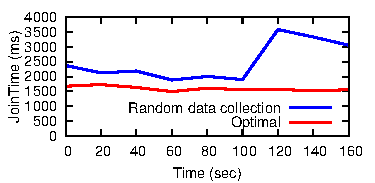
\includegraphics[width=0.45\textwidth]{figures/pytheas-problem-of-epsilon-change-JOINTIME.pdf}
        \label{subfig:problem-of-epsilon:change}
}
%\hspace{-0.1cm}
\subfloat[Example B: Overload and oscillations between decisions due to periodic prediction.]
{
        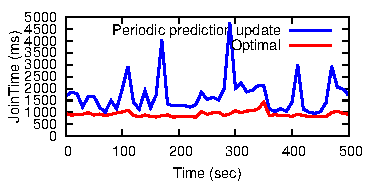
\includegraphics[width=0.45\textwidth]{figures/pytheas-problem-of-slow-load-JOINTIME.pdf}
        \label{subfig:problem-of-slow:load}
}
%\vspace{-0.2cm}
\caption{Limitations of prediction-oriented abstraction (e.g., CFA~\cite{cfa}) manifested in two real examples.}
%\vspace{-0.1cm}
\label{fig:abstraction}
\end{figure}


Many prior approaches (e.g.,~\cite{c3,cfa,cs2p,footprint}) 
for data-driven QoE optimization use a {\em prediction-based} 
workflow.  
That is, they periodically train a quality prediction model 
based on  passive measurements to inform decisions for 
future sessions; e.g., using history data to decide what 
will be  the best relay server for a Skype call or the best 
CDN for a video session?   
While such prediction-based approaches have proved useful, 
they suffer from well-known limitations, namely, 
{\em prediction bias} and {\em slow reaction}
~\cite{he2009learning,spand}.  
Next, we  highlight these issues using  CDN selection in 
video streaming as a concrete use case.% to highlight these effects.  

\subsection{Limitation 1: Prediction Bias}
A well-known problem of prediction-based workflows is that the prediction can be 
biased by prior decisions. Because the input measurement data are based on 
previous set of best decisions, we will 
not have a reliable way to estimate the potential  quality improvements 
of other decisions in the future~\cite{spand}.
%A simple measurement method is to passively measure the observed quality.
% Unfortunately, this  will bias future quality predictions as measurements will only be 
% based on the previous set of best decisions and we will 
%have to no reliable way to estimate the potential  quality improvements with other decisions in the future~\cite{spand}.
%\footnote{
% There could be other  systematic biases with passive measurements as well if there are hidden confounding factors. For instance, 
%  Google Hangouts uses relay servers only when a direct peer-to-peer connection is unavailable~\cite{hangouts-policy}. 
% However, sessions where the direct connection
% failed could have  intrinsically different behaviors (e.g., different connection types) from other sessions and thus estimating relay 
% performance from these measurements may provide incorrect predictions. }
A simple solution is to use a fixed percentage of sessions to explore 
different decisions. This could eliminate the above prediction bias.
However, it can still be suboptimal, since it might either let too many sessions  use suboptimal decisions when quality is stable, or collect insufficient data in presence of higher variance.

\smallskip \noindent\underline{Example A:}
Figure~\ref{subfig:problem-of-epsilon:change} shows a trace-driven evaluation to highlight such 
prediction biases. We use a trace of one of the major video providers in US. As a baseline, we consider prior work called CFA~\cite{cfa}, which uses a fixed fraction of 10\% sessions to randomly explore suboptimal decisions.\footnote{The process begins by assigning sessions uniformly at random to all decisions in the first minute, and after that, it assigns 90\% sessions to the optimal decisions based on the last minute.}
 We see that it leads to worse average video startup latency, or join time,
 than an optimal strategy that always picks the CDN with the best average quality in each minute.
Each video session can pick CDN1 or CDN2, and in the hindsight, CDN1 is on average better CDN2, except between t=40 and t=120,
 when CDN2 has a large variance.
 Even when CDN1 is consistently better than CDN2, CFA is worse than optimal, since it always assigns 10\% of sessions to use CDN2. 
 At the same time, when CDN2 becomes a better choice, CFA 
cannot detect this change in a timely fashion 
as  10\% is too small a fraction to reliably estimate quality of CDN2.

%Figure~\ref{fig:problem-of-epsilon} compares the quality of $\epsilon$-greedy with the optimal quality if we always pick the CDN with the best average quality.
%In Figure~\ref{subfig:problem-of-epsilon:stable}, CDN1 is constantly better than CDN2. 
%Since $\epsilon$-greedy always assigns 10\% of sessions to CDN2, quality of $\epsilon$-greedy is always substantially worse than optimal.
%In Figure~\ref{subfig:problem-of-epsilon:change}, CDN1 is better CDN2, except between 40 and 120 second, when CDN2 has a large variance and is better than CDN1.
%However, CFA could not identify the quality shift timely, because 10\% sessions are too few to reliably estimate quality of CDN2.
%In short, simple random data collection will either let too many sessions to use suboptimal decisions when quality is stable, or collect insufficient data when quality changes.

%\begin{figure*}[t!]
%\captionsetup[subfigure]{justification=centering,farskip=-1pt,captionskip=5pt}
%\centering
%\hspace{-0.5cm}
%\subfloat[Prediction-oriented abstraction]
%{
%        \includegraphics[width=0.35\textwidth]{figures/abstraction-prediction.pdf}
%        \label{subfig:abstraction-prediction}
%}
%\hspace{0.4cm}
%\subfloat[Real-time \mablong (\mab)]
%{
%        \includegraphics[width=0.35\textwidth]{figures/abstraction-mab.pdf}
%        \label{subfig:abstraction-mab}
%}
%\hspace{-0.5cm}
%\vspace{-0.1cm}
%\tightcaption{Comparing the traditional prediction-oriented abstraction with our abstraction of real-time \mab.}
%\vspace{-0.2cm}
%\label{fig:abstraction}
%\end{figure*}



\subsection{Limitation 2: Slow Reaction}
Due to the time taken to aggregate sufficient data for model building, 
today's prediction-based systems update quality predictions periodically on
coarse timescales; e.g., CFA updates models every tens of seconds~\cite{cfa}, and VIA updates its models every several hours~\cite{via}. 
%\cameraremove{\myparatight{Model drift}}
%Unfortunately, 
This  means that they cannot quickly adapt to changes in
operating conditions which can cause {\em model drifts}.  First, if there are
sudden quality changes (e.g., network congestion and service outage),
prediction-based approaches might result in suboptimal quality due to its slow reaction.  Furthermore, such model shifts might indeed be a
consequence of the slow periodic predictions; e.g., the best predicted server
or CDN will receive more requests and its performance may degrade
as its load increases.

\smallskip \noindent\underline{Example B:} We consider an AS and two CDNs. 
For each CDN, if it receives most sessions from the AS, it will be overloaded, and the sessions served by it will have bad quality.
Figure~\ref{subfig:problem-of-slow:load} shows that CFA, which always picks the CDN that has the best quality in the last minute, has worse quality than another
 strategy which assigns half of sessions to each CDN.  This is because 
 CFA always overloads the CDN that has the best historical performance by assigning most sessions to it, and CFA will switch decisions only {\em after} quality
degradation occurs, leading to oscillations and suboptimal quality.



At a high level,  these  limitations of prediction-based
approaches arise from the  logical
separation between measurement collection and decision making. Next, we discuss
what the right abstraction for data-driven QoE optimization should be to avoid
 these limitations.
